\documentclass{article}
\usepackage{blindtext}
\usepackage[utf8]{inputenc}
\usepackage{amsmath,bm}
\usepackage{amstext}
\usepackage{amsfonts}
\usepackage{amsmath}
\usepackage{multirow}
\usepackage{enumerate}
\usepackage{xeCJK}
\setCJKmainfont{STKaiti}
\usepackage{algorithm}
\usepackage{algorithmic}
\renewcommand{\algorithmicrequire}{ \textbf{输入:}} %Use Input in the format of Algorithm
\renewcommand{\algorithmicensure}{ \textbf{输出:}} %UseOutput in the format of Algorithm
\usepackage{graphicx}
\usepackage{booktabs}
\usepackage{listings}
\lstset{
	columns=fixed,       
	numbers=left,                                        % 在左侧显示行号
	numberstyle=\tiny\color{gray},                       % 设定行号格式
	frame=none,                                          % 不显示背景边框
	keywordstyle=\color[RGB]{40,40,255},                 % 设定关键字颜色
	numberstyle=\footnotesize\color{darkgray},           
	commentstyle=\it\color[RGB]{0,96,96},                % 设置代码注释的格式
	stringstyle=\rmfamily\slshape\color[RGB]{128,0,0},   % 设置字符串格式
	showstringspaces=false,                              % 不显示字符串中的空格
	language=python,                                        % 设置语言
}

\title{Neural Network and Applications\\Homework 3}
\author{陈轶洲 MF20330010}
\begin{document}
	\maketitle
	\numberwithin{equation}{section}
\section{}
不可以用$y = \left\{
\begin{aligned}
	0 \quad x \textless 0\\
	1 \quad x \ge 0
\end{aligned} 
\right. $来作为神经网络的激活函数,这是因为激活函数需要满足如下性质:
\begin{enumerate}[1)]
	\item 非线性:即导数不是常数,这是多层神经网络的基础,保证多层神经网络不退化成单层线性网络;
	\item 几乎处处可微:可微性保证了在优化中梯度的可计算性;
	\item 非饱和性:饱和指的是在某些区间梯度接近于零(即梯度消失),使得参数无法继续更新的问题;
\end{enumerate}
对于题干中所给激活函数,其不满足非线性和非饱和性,因为它在所有位置的梯度都为0,因此处处饱和,无法作为激活函数。



\section{}
首先对待求参数进行形式化定义:
\begin{equation}
	\begin{aligned}
	X&=\begin{bmatrix}i_1\\i_2\end{bmatrix}\quad W_1=\begin{bmatrix}w_1& w_2\\w_3 & w_4\end{bmatrix}\quad \\B&=\begin{bmatrix}b_1\\b_2\end{bmatrix}\quad W_2=\begin{bmatrix}w_5\\w_6\end{bmatrix}
	\end{aligned}
\end{equation}
接着用流程图直观表达前向传播过程:
\begin{figure}[H]
	\centering
	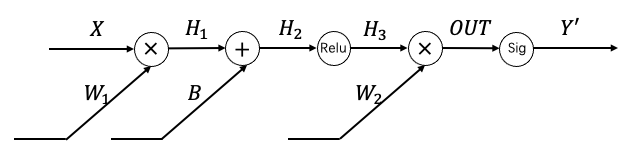
\includegraphics[scale=0.7]{forward.png}
\end{figure}
由上图可知前向传播的计算过程:
\begin{equation}
	\begin{aligned}
	H_1 &= W_1^TX\\
	H_2 &= H_1+B\\
	H_3 &= Relu(H_2)\\
	OUT &= W_2^TH_3\\
	Y' &= Sigmoid(OUT)
	\end{aligned}
\end{equation}
反向传播过程中的流程图如下所示:
\begin{figure}[H]
	\centering
	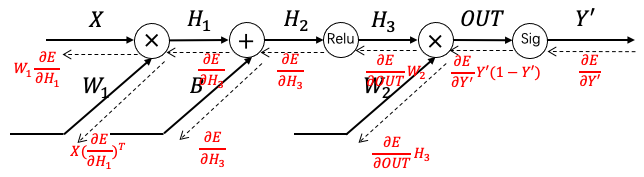
\includegraphics[scale=0.7]{backward.png}
\end{figure}
由式(2.2)可推出反向传播过程中各参数对损失函数的偏导,(将mask()定义为:找到原矩阵中非正元素位置,将其对应偏导矩阵中对应位置的元素置为0):
\begin{equation}
	\begin{aligned}
		\frac{\partial{E}}{\partial{Y'}}&=\frac{\partial{(Y'-Y)^2}}{\partial{Y'}}=2(Y'-Y)\\
		\frac{\partial{E}}{\partial{OUT}}&=\frac{\partial{E}}{\partial{Y'}}Y'(1-Y')=2(Y'-Y)Y'(1-Y')\\
		\frac{\partial{E}}{\partial{H_3}}&=	\frac{\partial{E}}{\partial{OUT}}W_2=2(Y'-Y)Y'(1-Y')W_2\\
		\frac{\partial{E}}{\partial{W_2}}&=	\frac{\partial{E}}{\partial{OUT}}H_3=2(Y'-Y)Y'(1-Y')H_3\\
		\frac{\partial{E}}{\partial{H_2}}&=mask(2(Y'-Y)Y'(1-Y')W_2)\\
		\frac{\partial{E}}{\partial{H_1}}&=mask(2(Y'-Y)Y'(1-Y')W_2)\\
		\frac{\partial{E}}{\partial{B}}&=mask(2(Y'-Y)Y'(1-Y')W_2)\\
		\frac{\partial{E}}{\partial{W_1}}&=X(\frac{\partial{E}}{\partial{H_1}})^T=X(mask(2(Y'-Y)Y'(1-Y')W_2))^T\\
		\frac{\partial{E}}{\partial{X}}&=W_1\frac{\partial{E}}{\partial{H_1}}=W_1mask(2(Y'-Y)Y'(1-Y')W_2)
	\end{aligned}
\end{equation}

以上就是对该神经网络前向与反向传播的完整推导。损失函数对于$ w_1,b_2,w_5 $的偏导,其表达式已被包含在了更抽象的$ \frac{\partial{E}}{\partial{W_1}}, \frac{\partial{E}}{\partial{B}},\frac{\partial{E}}{\partial{W_2}}$之中。特别的,当
$  X=\begin{bmatrix}0.3\\2.8\end{bmatrix}, W_1=\begin{bmatrix}0.4& 0.5\\0.2 & 0.4\end{bmatrix}, B=\begin{bmatrix}0.3\\0.8\end{bmatrix}, W_2=\begin{bmatrix}3.5\\0.6\end{bmatrix}$时:\\
前向传播:
\begin{equation}
	\begin{aligned}
		H_1 &= W_1^TX =\begin{bmatrix}0.68\\1.27\end{bmatrix}\\
		H_2 &= H_1+B=\begin{bmatrix}0.98\\2.07\end{bmatrix}\\
		H_3 &= Relu(H_2)=\begin{bmatrix}0.98\\2.07\end{bmatrix}\\
		OUT &= W_2^TH_3=\begin{bmatrix}4.672\end{bmatrix}\\
		Y' &= Sigmoid(OUT)=\begin{bmatrix}0.99073313\end{bmatrix}
	\end{aligned}
\end{equation}
反向传播:
\begin{equation}
	\begin{aligned}
		\frac{\partial{E}}{\partial{Y'}}&=\frac{\partial{(Y'-Y)^2}}{\partial{Y'}}=2(Y'-Y)=-9.21853373\\
		\frac{\partial{E}}{\partial{W_2}}&=	\frac{\partial{E}}{\partial{OUT}}H_3=2(Y'-Y)Y'(1-Y')H_3=\begin{bmatrix}-0.08294257\\ -0.17519502\end{bmatrix}\\
		\frac{\partial{E}}{\partial{B}}&=mask(2(Y'-Y)Y'(1-Y')W_2)=\begin{bmatrix}-0.29622346\\ -0.05078116\end{bmatrix}\\
		\frac{\partial{E}}{\partial{W_1}}&=X(\frac{\partial{E}}{\partial{H_1}})^T=X(mask(2(Y'-Y)Y'(1-Y')W_2))^T=\begin{bmatrix}-0.08886704 & -0.01523435\\-0.82942569 & -0.14218726\end{bmatrix}\\
	\end{aligned}
\end{equation}
损失函数对$w_3$的偏导为-0.83

\section{}
使用单神经元无法拟合二次曲线,这是因为单神经元只能拟合一次线性曲线,而二次曲线是非线性的。\\
为了拟合二次曲线,至少需要三个神经元,如下图所示:
\begin{figure}[H]
	\centering
	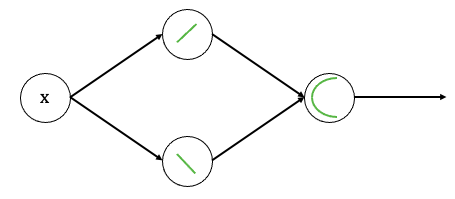
\includegraphics[scale=0.7]{neural.png}
\end{figure}
已知单神经元只能拟合线性函数,所以在隐藏层中使用两个神经元,用来拟合两条直线,输出层使用一个神经元将隐藏层训练的两条线连接起来,达到拟合二次曲线的目的。

\end{document}